\section{Esquematização do conteúdo das páginas}

De forma a ser possível entender que dados serão necessários para alimentar o software, o que apresentar em 
cada página e também como navegar entre os ecrãs da aplicação foi então desenhado um esquema 
(Figura~\ref{fig:3}).

\begin{figure}[htb]
    \centering
    
    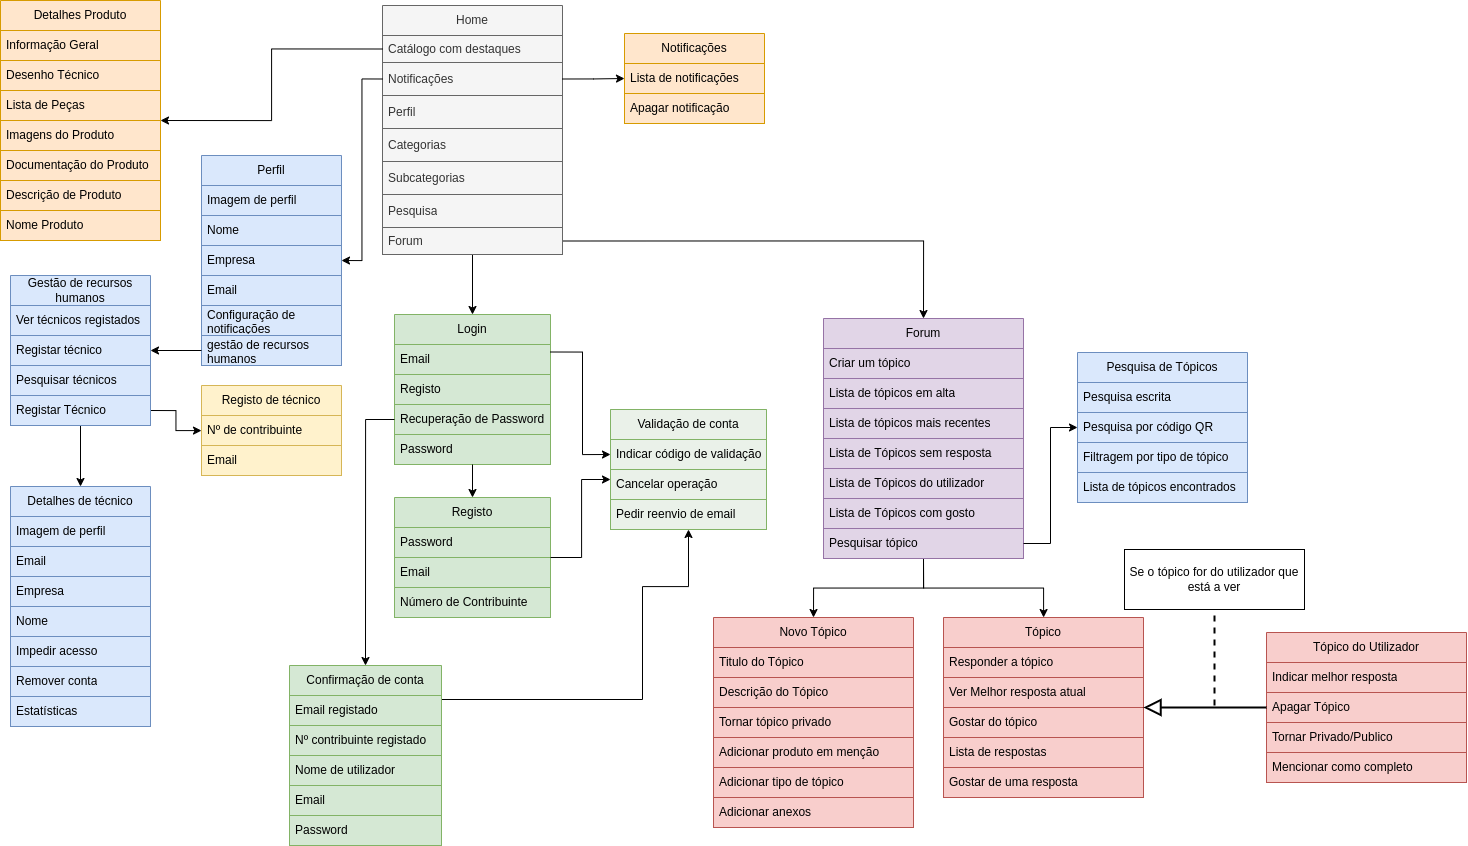
\includegraphics[width=\textwidth]{images/Arquiteturas/diagrama_superficial_de_aplicacao.png}
    \caption{Esquema de organização de páginas do software}
    \label{fig:3}
\end{figure}

\newpage

\subsection{Autenticação e página Inicial}

Através deste esquema é possível perceber que através do ecrã principal o utilizador tem acesso ao 
catálogo de produtos e ao fórum, neste o utilizador pode também realizar o login e o logout que 
redirecionam para os respetivos ecrãs.

O ecrã de login é então necessário o utilizador indicar o número de contribuinte e a password, neste ele 
pode também pedir recuperação de password e/ou redirecionar para o registo onde necessitará de número de 
contribuinte, password e email para o realizar.

Em caso de o utilizador não possuir a sua conta ativa, este será encaminhado para o ecrã de validar conta 
em que poderá indicar o código de validação, cancelar a operação voltando para o ecrã anterior e pedir o 
reenvio do código de validação.

Em caso de se tratar de um técnico que necessita de confirmar a sua conta, este conseguirá ver as 
informações registadas e introduzir o seu nome, alterar o seu email e password.

\begin{figure}[htb]
    \centering
    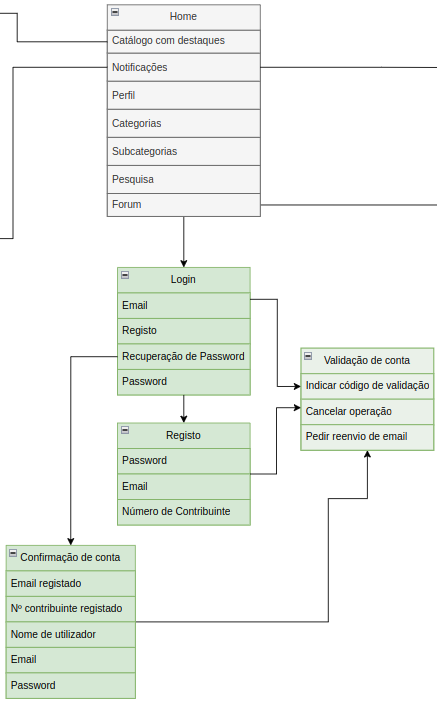
\includegraphics[height=0.9\textwidth]{images/Arquiteturas/superficial_de_app/home_auth.png}
    \caption{Esquema de organização das páginas de autenticação e página inicial}
    \label{fig:4}
\end{figure}

\newpage

\subsection{Fórum}

Através do ecrã inicial o utilizador pode se direcionar para o ecrã de fórum, neste ecrã ele poderá pesquisar
 por tópicos, ou então aceder a tópicos em alta, tópicos mais recentes, tópicos sem resposta e pesquisar tópicos.
O técnico consegue também ver os seus tópicos e criar tópicos.

\begin{figure}[htb]
    \centering
    
    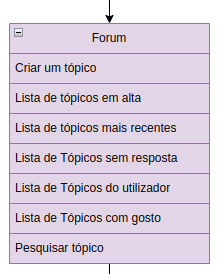
\includegraphics[height=0.4\textwidth]{images/Arquiteturas/superficial_de_app/forum.png}
    \caption{Esquema de organização da página de fórum}
    \label{fig:5}
\end{figure}

\subsection{Criar novo tópico}

Quando o técnico decide criar um tópico ele tem de indicar o título e a descrição do seu tópico, de seguida 
poderá indicar se o tópico é privado ou não, indicar o tipo de tópico, o produto referente e adicionar 
anexos.

\begin{figure}[htb]
    \centering
    
    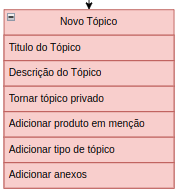
\includegraphics[height=0.3\textwidth]{images/Arquiteturas/superficial_de_app/criar_topico.png}
    \caption{Esquema de organização da pagina de criação de tópico}
    \label{fig:6}
\end{figure}

\newpage

\subsection{Detalhes de tópico}

O utilizador pode também ver os detalhes do tópico, já o técnico pode também responder a um tópico, 
gostar do tópico, gostar de uma resposta.
Caso este tópico seja do mesmo, este pode indicar a melhor resposta, apagar o tópico, tornar o tópico 
público ou privado e mencionar como completo.

\begin{figure}[htb]
    \centering
    
    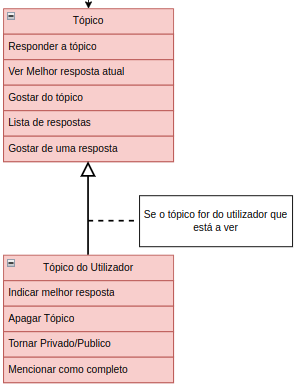
\includegraphics[height=0.55\textwidth]{images/Arquiteturas/superficial_de_app/detalhes_topico.png}
    \caption{Esquema de organização da página de detalhes de tópico}
    \label{fig:7}
\end{figure}

\subsection{Pesquisa de tópicos}

A página de pesquisa permite ao utilizador pesquisar por tópicos específicos tanto pesquisando por nome como 
por código QR de um produto. Para além da pesquisa o utilizador pode também realizar a filtragem dos 
tópicos por tipo.
\begin{figure}[htb]
    \centering
    
    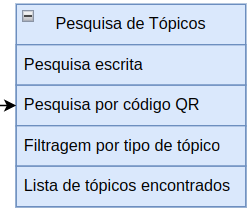
\includegraphics[height=0.3\textwidth]{images/Arquiteturas/superficial_de_app/pesquisa_forum.png}
    \caption{Esquema de organização da página de pesquisa de tópicos}
    \label{fig:8}
\end{figure}

\subsection{Notificações}

A página de notificações permite ao técnico visualizar as suas notificações, assim como também apagar estas.
\begin{figure}[htb]
    \centering
    
    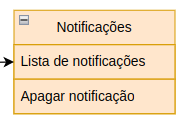
\includegraphics[height=0.2\textwidth]{images/Arquiteturas/superficial_de_app/notificacoes.png}
    \caption{Esquema de organização da página de notificações}
    \label{fig:9}
\end{figure}

\subsection{Perfil}

A página de perfil de técnico permite a este visualizar as suas informações, assim como alterar 
o seu email e configurar as notificações do mesmo. Caso se trate de uma empresa a visualizar o seu perfil,
esta poderá ter acesso à gestão de recursos humanos, para gerir os seus técnicos.
\begin{figure}[htb]
    \centering
    
    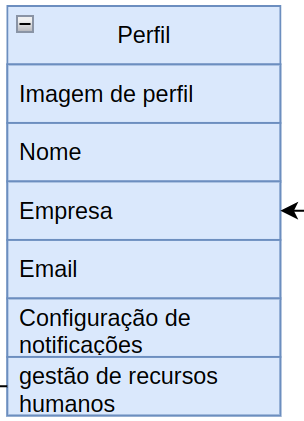
\includegraphics[height=0.35\textwidth]{images/Arquiteturas/superficial_de_app/perfil.png}
    \caption{Esquema de organização da página de notificações}
    \label{fig:10}
\end{figure}

\newpage

\subsection{Gestão de recursos humanos}

A página de perfil gestão de recursos humanos permite à empresa gerir todos os seus técnicos registados 
e criar contas de técnicos. Assim que a empresa seleciona um técnico, esta verá o seu perfil, 
com estatísticas do técnico
\begin{figure}[htb]
    \centering
    
    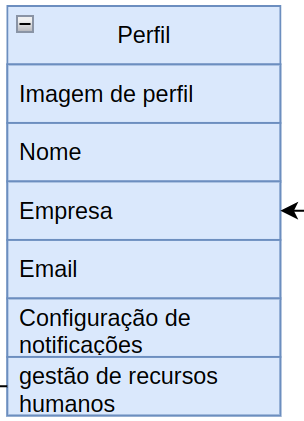
\includegraphics[height=0.35\textwidth]{images/Arquiteturas/superficial_de_app/perfil.png}
    \caption{Esquema de organização da página de gestão de recursos humanos}
    \label{fig:11}
\end{figure}